\chapter{Localization}

\begin{recall}
    A subset $U \subseteq R$ is \emph{multiplicatively closed} if $1 \in U$ and for $u,v \in U$, $uv \in U$, 
\end{recall}

\begin{example}
    \begin{enumerate}
        \item $\{1,f,f^2,\cdots\} \subseteq R$ is multiplicatively closed for $f \in R$.
        \item $R^\times \subseteq R$ is multiplicatively closed.
        \item $R \setminus \ffp \subseteq R$ is multiplicatively closed for $\ffp \in \operatorname{Spec}(R)$.
        \item $1 + \ffa \subseteq R$ is multiplicatively closed for $\ffa \leq R$.
    \end{enumerate}
\end{example}

\begin{recall} \label{defOfMultiplicativelyClosedSet}
    For $U \subseteq R$ multiplicatively closed, $U^{-1}R = \{\frac{r}{u} \mid r \in R, u \in U\}$, where $\frac{r}{u} = \frac{r'}{u'}$ if and only if there exists $u'' \in U$ such that $u''(ru'-r'u) = 0$, i.e., $\frac{u''r}{u''u} = \frac{r'}{u'}$, formally, $\frac{r}{u}$ is the equivalence class under an equivalence relation. \par 
    $U^{-1}R$ is a nonzero commutative ring with identity with $\frac{r}{u} + \frac{s}{v} = \frac{rv+su}{uv}$ and $\frac{r}{u} \frac{s}{v} = \frac{rs}{uv}$ for $\frac{r}{u},\frac{s}{v} \in U^{-1}(R)$. \par 
    $0_{U^{-1}(R)} = \frac{0_R}{1_R} = \frac{0}{u}$ and $1_{U^{-1}R} = \frac{1_{R}}{1_{R}} = \frac{u}{u}$ for all $u \in U$. \par 
    $\frac{r}{u} = 0$ if and only if there exists $u'' \in U$ such that $u''r = 0$. \par 
    $\psi: R \to U^{-1}R$ given by $\psi(r) = \frac{r}{1}$ is a well-defined ring homomorphism.
\end{recall}

\begin{notation}
    \begin{enumerate}
        \item If $U = \{1,f,f^2,\cdots\}$, write $U^{-1}R = R_f$.
        \item If $U = R \setminus \ffp$ for some $\ffp \in \operatorname{Spec}(R)$, write $U^{-1}R = R_\ffp$.
        \item If $U \subseteq R$ is multiplicatively closed, write $U^{-1}R = R_U = R[U^{-1}]$.
    \end{enumerate}
\end{notation}

\noindent Let $U \subseteq R$ multiplicatively closed.

\begin{customrecall}{\ref{defOfMultiplicativelyClosedSet}+$\epsilon$}
    For $u \in U$, $\psi(u) \in (U^{-1}R)^{\times}$ since $\frac{1}{u} = (\frac{u}{1})^{-1} = (\psi(u))^{-1}$.
\end{customrecall}

\begin{proposition}[UMP for $\psi$]
    Let $\varphi: R \to S$ be a ring homomorphism such that $\varphi(U) \subseteq S^{\times}$. Then there exists a unique ring homomorphism $\Phi:U^{-1}R \to S$ such that $\Phi \circ \psi = \varphi$. In fact, $\Phi(\frac{r}{u}) = \varphi(r)\varphi(u)^{-1}$ for $\frac{r}{u} \in U^{-1}R$.
    \begin{center}
        \begin{tikzcd}
            R \rar["\psi"] \drar["\varphi"'] & U^{-1}R \dar[dashed,"\ex !\ \Phi"] \\
            & S
        \end{tikzcd}
    \end{center}
\end{proposition}

\begin{proof}
    Let $\frac{r}{u} = \frac{r'}{u'}$. Then there exists $u'' \in U$ such that $u''(ru'-r'u) = 0$. Since $\varphi$ is a ring homomorphism, we have $\varphi(u'')(\varphi(r)\varphi(u') - \varphi(r')\varphi(u)) = 0$. Also, since $\varphi(u'') \in S^{\times}$, we have $\varphi(r)\varphi(u') = \varphi(r')\varphi(u)$, i.e., $\varphi(r)\varphi(u)^{-1} = \varphi(r')\varphi(u')^{-1}$ since $\varphi(u), \varphi(u') \in S^{\times}$. So $\phi$ is well-defined. \par
    Since $\Phi(\frac{r}{u} + \frac{s}{v}) = \Phi(\frac{rv+su}{uv}) = \varphi(rv+su)\varphi(uv)^{-1} = (\varphi(r)\varphi(v) + \varphi(s)\varphi(u))) \varphi(u)^{-1}\varphi(v)^{-1} = \varphi(r)\varphi(u)^{-1} + \varphi(s)\varphi(v)^{-1} = \Phi(\frac{r}{u}) + \Phi(\frac{s}{v})$ and similarly, $\Phi(\frac{r}{u} \cdot \frac{s}{v}) = \Phi(\frac{r}{u})\Phi(\frac{s}{v})$ for $\frac{r}{u},\frac{s}{v} \in U^{-1}R$, we have $\Phi$ is ring homomorphism. \par 
    Suppose there is another ring homomorphism $\Lambda: U^{-1}R \to S$ such that $\Lambda \circ \psi = \varphi$.
    \begin{center}
        \begin{tikzcd}
            R \rar["\psi"] \drar["\varphi"'] & U^{-1}R \dar["\Lambda"] \\
            & S
        \end{tikzcd}
    \end{center}
    Then $\varphi(r) = \Lambda (\psi(r)) = \Lambda (\frac{r}{1})$ for $r \in R$. So $\Lambda(\frac{r}{u}) = \Lambda(\frac{r}{1} \frac{1}{u}) = \Lambda(\frac{r}{1}) \Lambda(\frac{u}{1})^{-1} = \varphi(r) \varphi(u)^{-1} = \Phi(\frac{r}{u})$ for $\frac{r}{u} \in U^{-1}R$. Thus, $\Lambda = \Phi$, i.e., such $\Phi$ is unique.
\end{proof}

\begin{proposition}
    Let $\varphi: R \to S$ be a ring homomorphism.
    \begin{enumerate}
        \item $\varphi(U) \subseteq S$ is multiplicatively closed and $\varphi(U)^{-1}S =: U^{-1}S$.
        \item There is a ring homomorphism: $U^{-1}\varphi: U^{-1}R \to U^{-1}S$ given by $U^{-1}\varphi(r/u) = \varphi(r)/\varphi(u)$.
            \begin{center}
                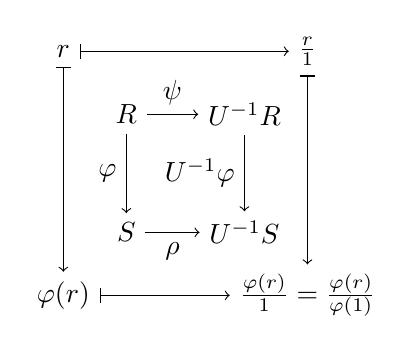
\begin{tikzpicture}[node distance = 1.5cm, auto]
                    \node (R) {$R$};
                    \node (UR)[right of=R] {$U^{-1}R$};
                    \node (S)[below of=R] {$S$};
                    \node (US)[below of=UR] {$U^{-1}S$};
                    \node (r)[node distance=0.8cm, left of=R, above of=R] {$r$};
                    \node (ur)[node distance=0.8cm, right of=UR, above of=UR] {$\frac{r}{1}$};
                    \node (s)[node distance=0.8cm, left of=S, below of=S] {$\varphi(r)$};
                    \node (us)[node distance=0.8cm, right of=US, below of=US] {$\frac{\varphi(r)}{1} = \frac{\varphi(r)}{\varphi(1)}$};
                    \draw[->] (R) to node {$\psi$} (UR);
                    \draw[->] (R) to node [swap]{$\varphi$} (S);
                    \draw[->] (UR) to node [swap] {$U^{-1}\varphi$} (US);
                    \draw[->] (S) to node [swap]{$\rho$} (US);
                    \draw[|->] (r) to node {} (ur);
                    \draw[|->] (r) to node {} (s);
                    \draw[|->] (s) to node {} (us);
                    \draw[|->] (ur) to node {} (us);
                \end{tikzpicture}
            \end{center}
        \item If $\varphi$ is onto, $U^{-1}\varphi$ is onto.
        \item If $\varphi$ is 1-1, $U^{-1}\varphi$ is 1-1.
        \item If $\alpha: S \to T$ is a ring homomorphism, then $U^{-1}(\alpha \circ \varphi) = (\varphi(U)^{-1}\alpha) \circ (U^{-1}\varphi)$. 
        \begin{center}
            \begin{tikzpicture}[node distance = 1.5cm, auto]
                \node (S) {$S$};
                \node (US)[node distance=3cm, right of=S] {$U^{-1}S$};
                \node (R)[above of=S, left of=S] {$R$};
                \node (T)[below of=S, left of=S] {$T$};
                \node (UR)[above of=S, right of=S] {$U^{-1}R$};
                \node (UT)[below of=S, right of=S] {$\varphi(U)^{-1}T$};

                \node [node distance=2cm, right of=UT] {$:=\alpha (\varphi(U))^{-1}T$};
                \node [node distance=1.45cm, right of=US] {$:=\varphi(U)^{-1}S$};
                \draw[->] (R) to node {$\varphi$} (S);
                \draw[->] (R) to node [swap]{$\alpha \circ \varphi$} (T);
                \draw[->] (S) to node {$\alpha$} (T);
                \draw[->] (R) to node {$\psi$} (UR);
                \draw[->] (T) to node {} (UT);
                \draw[->] (UR) to node {$U^{-1}\varphi$} (US);
                \draw[->] (US) to node {} (UT);
                \node (zzz)[node distance=0.8cm, below of=US] {$\varphi(U)^{-1} \alpha$};
                \draw[->,name path=line 1] (S) to node {} (US);
                \path[name path=line 2] (UR) to node {} (UT);
                % find intersection of first and second line
                \path [name intersections={of = line 1 and line 2}];
                \coordinate (P)  at (intersection-1);

                % path a circle around this intersection for the arc
                \path[name path=circle] (P) circle(1.mm);
                % find intersections of second line and circle
                \path [name intersections={of = circle and line 2}];
                \coordinate (I1)  at (intersection-1);
                \coordinate (I2)  at (intersection-2);
                % draw normal line segments
                \draw (UR) -- (I1);
                \draw[->] (I2) -- (UT);
                % draw arc at intersection
                \tkzDrawArc[color=black](P,I1)(I2);
            \end{tikzpicture}
        \end{center}
    \end{enumerate}
\end{proposition}

\begin{proof}
    \begin{enumerate}
        \item [(b)] 
            Let $\frac{r}{u} = \frac{r'}{u'} \in U^{-1}R$. Then there exists $u'' \in U$ such that $u''(ur'-u'r) = 0$. So there exists $\varphi(u'') \in \varphi(U)$ such that $\varphi(u'')(\varphi(r)\varphi(u') - \varphi(r')\varphi(u)) = 0$. Hence $\frac{\varphi(r)}{\varphi(u)} = \frac{\varphi(r')}{\varphi(u')} \in U^{-1}S$. \par  
            Since $U^{-1}\varphi(\frac{r}{u} + \frac{s}{v}) = U^{-1}\varphi(\frac{rv+su}{uv}) = \frac{\varphi(rv+su)}{\varphi(uv)} = \frac{\varphi(r)\varphi(v)+\varphi(s)\varphi(u)}{\varphi(u)\varphi(v)} = \frac{\varphi(r)}{\varphi(u)}+\frac{\varphi(s)}{\varphi(v)} = U^{-1}\varphi(\frac{r}{u})+U^{-1}(\varphi)(\frac{s}{v})$ and similarly, $U^{-1}(\varphi)(\frac{r}{u} \cdot\frac{s}{v}) = U^{-1}\varphi(\frac{r}{u})U^{-1}\varphi(\frac{s}{v})$ for $\frac{r}{u},\frac{s}{v} \in U^{-1}R$, we have $U^{-1}\varphi$ is a ring homomorphism. 
        \item [(c)]
            Assume $\varphi$ is onto. Let $\frac{s}{\varphi(u)} \in U^{-1}S$. Then there exists $r \in R$ such that $\varphi(r) = s$. Since $U^{-1}\varphi(\frac{r}{u}) = \frac{\varphi(r)}{\varphi(u)} = \frac{s}{\varphi(u)}$, we have $U^{-1}\varphi$ is onto.
        \item[(d)] Assume $\varphi$ is 1-1. Let $\frac{r}{u} \in U^{-1}R$. Then $\frac{r}{u} \in \ker(U^{-1}\varphi)$ if and only if $0 = U^{-1}\varphi(\frac{r}{u}) = \frac{\varphi(r)}{\varphi(u)}$ if and only if there exists $u'' \in U$ such that $\varphi(u'')\varphi(r) = 0 = \varphi(u''r)$ if and only if there exists $u'' \in U$ such that $u''r = 0$ if and only if $\frac{r}{u} = 0$ in $U^{-1}R$. Also, by (b) we have $U^{-1}\varphi$ is 1-1.
        \item[(e)]
            Since $\varphi:R \to S$ and $\alpha: S \to T$ are ring homomorphisms, $\alpha \circ \varphi$ is a ring homomorphism. Since $\alpha(\varphi(U)) \subseteq T$ is multiplicatively closed by (a), $\varphi(U)^{-1}\alpha$ is well-defined. 
        \[
            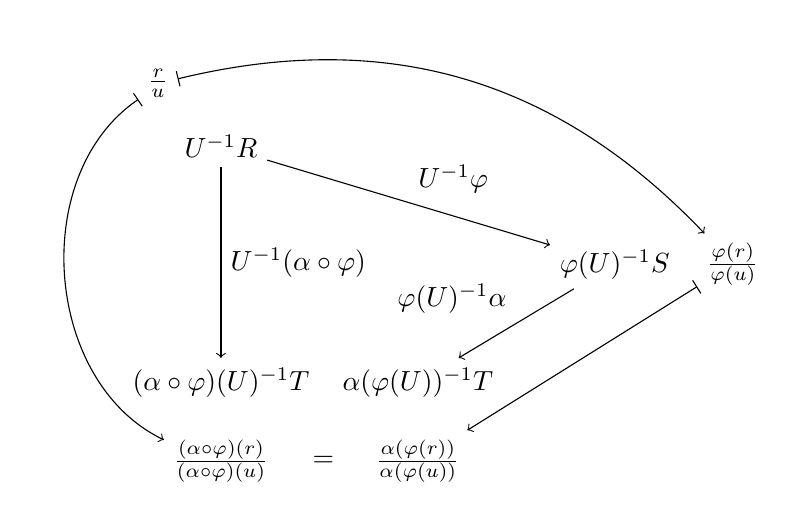
\begin{tikzpicture}[auto]
                \node (UR) {$U^{-1}R$};
                \node (UT)[node distance=3cm, below of=UR] {$(\alpha \circ \varphi)(U)^{-1}T$};
                \node (XXX)[node distance=1.5cm, below of=UR] {};
                \node (US)[node distance=5cm, right of=XXX] {$\varphi(U)^{-1}S$};
                \node (UT2)[node distance=2.5cm, right of=UT] {$\alpha (\varphi(U))^{-1}T$};
                \draw[->] (UR) to node {$U^{-1}(\alpha \circ \varphi)$} (UT);
                \draw[->] (UR) to node {$U^{-1}\varphi$} (US);
                \draw[->] (US) to node [swap]{$\varphi(U)^{-1}\alpha$} (UT2);
                \node (ur) [node distance=0.8cm, above of=UR,left of=UR]{$\frac{r}{u}$};
                \node (ut) [node distance=1cm, below of=UT]{$\frac{(\alpha \circ \varphi)(r)}{(\alpha \circ \varphi)(u)}$};
                \node (ut2) [node distance=1cm, below of=UT2]{$\frac{\alpha(\varphi(r))}{\alpha(\varphi(u))}$};
                \node (us) [node distance=1.5cm, right of=US]{$\frac{\varphi(r)}{\varphi(u)}$};
                \draw[|->, bend left] (ur) to node {} (us);
                \draw[|->] (us) to node [swap]{} (ut2);
                \draw[|->, bend right=60] (ur) to node {} (ut); 
                \node (equal) [node distance=1.3cm, right of=ut] {$=$}; 
            \end{tikzpicture} \qedhere
        \]
    \end{enumerate}
\end{proof}

\begin{proposition}
    Let $\varphi:R \to S$ be a ring homomorphism and $\varphi(U) \subseteq S$ is multiplicatively closed. Then $\im(U^{-1}\varphi) \cong U^{-1} \im(\varphi)$.
\end{proposition}

\begin{proof}
    By Proposition 3.6(e), $\im(U^{-1}\varphi) = \im((\pi(U)^{-1}i) \circ U^{-1}\pi)$. Since $\pi$ is onto, $U^{-1}(\pi)$ is onto by Proposition 3.6(c). So $\im(U^{-1}\varphi) = \im((\pi(U)^{-1}i))$. Since $\pi$ is 1-1, $\pi(U)^{-1}i$ is 1-1 by Proposition 3.6(d). Hence by the first isomorphism theorem, $U^{-1}\im(\varphi) \cong \im(\pi(U)^{-1}i) = \im(U^{-1}\varphi)$.
    \begin{center}
        \begin{tikzpicture}[node distance = 1.5cm, auto]
            \node (Im) {$\im(\varphi)$};
            \node (UIm)[node distance=3cm, right of=Im] {$U^{-1}\im(\varphi)$};
            \node (R)[above of=Im, left of=Im] {$R$};
            \node (S)[below of=Im, left of=Im] {$S$};
            \node (UR)[above of=Im, right of=Im] {$U^{-1}R$};
            \node (US)[below of=Im, right of=Im] {$U^{-1}S$};
            \draw[->] (R) to node {$\pi$} (Im);
            \draw[->] (R) to node [swap]{$\varphi$} (S);
            \draw[->] (Im) to node {$i$} (S);
            \draw[->] (R) to node {$\psi$} (UR);
            \draw[->] (S) to node {} (US);
            \draw[->] (UR) to node {$U^{-1}\pi$} (UIm);
            \draw[->] (UIm) to node {} (US);
            \node (zzz)[node distance=0.85cm, below of=UIm] {$\pi(U)^{-1}i$};
            \node (www)[node distance=0.8cm, below of=UR] {};
            \node [node distance=0.55cm, left of=www] {$U^{-1}\varphi$};
            \draw[->,name path=line 1] (Im) to node {} (UIm);
            \path[name path=line 2] (UR) to node {} (US);
            % find intersection of first and second line
            \path [name intersections={of = line 1 and line 2}];
            \coordinate (P)  at (intersection-1);
            % path a circle around this intersection for the arc
            \path[name path=circle] (P) circle(1.mm);
            % find intersections of second line and circle
            \path [name intersections={of = circle and line 2}];
            \coordinate (I1)  at (intersection-1);
            \coordinate (I2)  at (intersection-2);
            % draw normal line segments
            \draw (UR) -- (I1);
            \draw[->] (I2) -- (US);
            % draw arc at intersection
            \tkzDrawArc[color=black](P,I1)(I2);
        \end{tikzpicture}
    \end{center}
\end{proof}

\noindent Let $\ffa,\ffb \leq R$.

\begin{definition}
    Define relation ``$\sim$'' on $U \times \ffa$: $(u,a) \sim (u',a')$ if and only if there exists $u'' \in U$ such that $u''(u'a - ua') = 0$.
\end{definition}

\begin{fact}
    This is an equivalence relation.
\end{fact}

\begin{notation}
    $U^{-1}\ffa = \{\text{equivalence classes from $U \times \ffa$ under $\sim$}\}$, and $a/u$ or $\frac{a}{u}$ with $a \in \ffa$ and $u \in U$ are its elements.
\end{notation}

\begin{proposition}
    \begin{enumerate}
        \item The map $i: U^{-1}\ffa \to U^{-1}R$ given by $i(a/u) = a/u$ is well-defined and 1-1. Identify $U^{-1}\ffa$ with $\im(i) \subseteq U^{-1}R$, so write $U^{-1}\ffa \subseteq U^{-1}R$. \\
            \textbf{Warning.} $\frac{r}{u} \in U^{-1}R$ such that $\frac{r}{u} \in U^{-1}\ffa$ may have $r \not \in \ffa$.
        \item If $\frac{r}{u} \in U^{-1}R$, then $\frac{r}{u} \in U^{-1}\ffa$ if and only if there exists $v \in U$ such that $vr \in \ffa$. 
        \item Let $\pi: R \to \frac{R}{\ffa}$ be the natural surjection. Then $U^{-1}\ffa = \ker(U^{-1} \pi) \leq U^{-1}R$ and $U^{-1}R/U^{-1}\ffa \cong U^{-1}\frac{R}{\ffa}$.
        \item More generally, if $\varphi: R \to S$ is a ring homomorphism, then $U^{-1} \ker(\varphi) = \ker(U^{-1}\varphi) \leq U^{-1}R$ such that $\im(U^{-1}\varphi) \cong U^{-1}R/U^{-1}\ker(\varphi)$.
        \item $U^{-1}\ffa = \ffa \cdot U^{-1}R$, extension of $\ffa$ along $\psi: R \to U^{-1}R$.
    \end{enumerate}
\end{proposition}

\begin{proof}
    \begin{enumerate}
        \item By the definition of ``$\sim$'', $i$ is well-defined. \par 
            Let $\frac{a}{u} \in U^{-1}\ffa$. Then $\frac{a}{u} \in \ker(i)$ if and only if $i(\frac{a}{u})=0$ in $U^{-1}R$ if and only if there exists $v \in U$ such that $va = 0$ in $R$ if and only if there exists $v \in U$ such that $va = 0$ in $\ffa$ if and only if $\frac{a}{u} = \frac{va}{vu} = \frac{0}{vu} = 0$ in $U^{-1}\ffa$. Also, since $i$ is a ring homomorphism, $i$ is 1-1.
        \item ``$\Rightarrow$''. Since $\frac{r}{u} \in U^{-1}\ffa$, $\frac{r}{u} = \frac{a}{u}$ for some $a \in \ffa$ in $U^{-1}R$. So there exists $u'' \in U$ such that $u''u'r = u''ua \in \ffa$. Let $v = u''u$. Then $vr \in \ffa$. \par 
            ``$\Leftarrow$''. Note $\frac{r}{u} = \frac{vr}{vu} \in U^{-1}\ffa$ since $vr \in \ffa$.
        \item By (d).
        \item Let $\frac{r}{u} \in U^{-1}R$. Then $\frac{r}{u} \in U^{-1}\ker(\varphi)$ if and only if there exists $v \in U$ such that $vr \in \ker(\varphi)$ by (a) if and only if there exists $\varphi(v) \in \varphi(U)$ such that $\varphi(vr) = 0 = \varphi(v)\varphi(r)$ if and only if $U^{-1}\varphi(\frac{r}{u}) = \frac{\varphi(r)}{\varphi(u)} = 0$ in $U^{-1}S = \varphi(U)^{-1}S$ if and only if $\frac{r}{u} \in \ker(U^{-1}\varphi)$. \par 
            By the first isomorphism theorem, $\im(U^{-1}\varphi) \cong U^{-1}R/\ker(U^{-1}\varphi) \cong U^{-1}R/U^{-1}\ker(\varphi)$.  
        \item 
            ``$\supseteq$''. It follows from $\ffa \cdot U^{-1}R$ is generated by $\psi(a) = \frac{a}{1} \in U^{-1}\ffa$. \par 
            ``$\subseteq$''. Let $\frac{a}{u} \in U^{-1}\ffa$. Then $\frac{a}{u} = \frac{a}{1} \cdot \frac{1}{u} = \psi(a) \cdot \frac{1}{u} \in \ffa \cdot U^{-1}R$. \qedhere
    \end{enumerate}
\end{proof}

\begin{proposition}
    \begin{enumerate}
        \item $U^{-1}(\ffa + \ffb) = (U^{-1}\ffa) + (U^{-1}\ffb)$.
        \item $U^{-1}(\ffa \cap \ffb) = (U^{-1}\ffa) \cap (U^{-1}\ffb)$.
        \item $U^{-1}(\ffa \ffb) = (U^{-1}\ffa) (U^{-1}\ffb)$.
        \item $U^{-1} \operatorname{rad}(\ffa) = \operatorname{rad}(U^{-1}\ffa)$.
        \item $U^{-1}\operatorname{Nil}(R) = \operatorname{Nil}(U^{-1}R)$.
        \item $U^{-1}(\ffb:\ffa) = (U^{-1}\ffb:U^{-1}\ffa)$  if $\ffa$ is finitely generated.
    \end{enumerate}
\end{proposition}

\begin{proof}
    \begin{enumerate}
        \item By Proposition 3.11(e) and 1.63(c), we have $U^{-1}(\ffa+\ffb) = (\ffa+\ffb) \cdot U^{-1}R = (\ffa \cdot U^{-1}R) + (\ffb \cdot U^{-1}R) = (U^{-1}\ffa) + (U^{-1}\ffb)$.
        \item ``$\subseteq$''. By Proposition 3.11(e) and 1.63(d), $U^{-1}(\ffa \cap \ffb) = (\ffa \cap \ffb) \cdot U^{-1}R \subseteq (\ffa \cdot U^{-1}R) \cap (\ffb \cdot U^{-1}R) = (U^{-1}\ffa) \cap (U^{-1}\ffb)$. \par 
            ``$\supseteq$''. Let $\frac{r}{u} \in U^{-1}R$ such that $\frac{r}{u} \in (U^{-1}\ffa) \cap (U^{-1}\ffb)$. Then there exist $v,w \in U$ such that $vr \in \ffa$ and $wr \in \ffb$ by Proposition 3.11(b). So $(vw)r \in \ffa \cap \ffb$. Also, since $vw \in U$, $\frac{r}{u} \in U^{-1}(\ffa \cap \ffb)$ by Proposition 3.11(b). 
        \item By Proposition 3.11(e) and 1.63(e), we have $U^{-1}(\ffa\ffb) = (\ffa\ffb) \cdot U^{-1}R = (\ffa \cdot U^{-1}R)(\ffb \cdot U^{-1}R) = (U^{-1}\ffa)(U^{-1}\ffb)$.
        \item ``$\subseteq$''. By Proposition 3.11(e) and 1.63(g), $U^{-1} \operatorname{rad}(\ffa) = \operatorname{rad}(\ffa) \cdot U^{-1}R \subseteq \operatorname{rad}(\ffa \cdot U^{-1}R) = \operatorname{rad}(U^{-1}\ffa)$. \par 
            ``$\supseteq$''. Let $\frac{r}{u} \in \operatorname{rad}(U^{-1}\ffa)$. Then $\frac{r^{n}}{u^{n}} = (\frac{r}{u})^{n} \in U^{-1}\ffa$ for some $n \geq 1$. So there exists $v \in U$ such that $vr^{n} \in \ffa$. Hence $(vr)^{n} = v^{n-1} \cdot vr^{n} \in \ffa$. So $vr \in \operatorname{rad}(\ffa)$. Thus, $\frac{r}{u} \in U^{-1} \operatorname{rad}(\ffa)$.
        \item Special case of (d) with $\ffa = 0$. 
        \item ``$\subseteq$''. By Proposition 3.11(e) and 1.63(f), $U^{-1}(\ffb:\ffa) = (\ffb:\ffa) \cdot U^{-1}R \subseteq (\ffb \cdot U^{-1}R: \ffa \cdot U^{-1}R) = (U^{-1}\ffb:U^{-1}\ffa)$. \par 
            ``$\supseteq$''. Let $\frac{r}{u} \in (U^{-1}\ffb:U^{-1}\ffa)$. Since $\ffa$ is finitely generated, $\ffa = \langle a_{1},\cdots,a_{n} \rangle R$ for some $n \geq 1$ and $a_{1},\cdots,a_{n} \in R$. Then $U^{-1}\ffa = \langle \frac{a_{1}}{1},\cdots,\frac{a_{n}}{1} \rangle U^{-1}R$. Since $\frac{r}{u} \in (U^{-1}\ffb:U^{-1}\ffa)$, $\frac{ra_{i}}{u} = \frac{r}{u} \frac{a_{i}}{1} \in U^{-1}\ffb$ for $i = 1,\cdots,n$. So there exists $v_{i} \in U$ such that $v_{i} ra_{i} \in \ffb$ for $i = 1,\cdots,n$. Let $v = v_{1} \cdots v_{n} \in U$. Then $(vr)a_{i} \in \ffb$ for $i = 1,\cdots,n$. So $vr \in (\ffb:\ffa)$. Thus, $\frac{r}{u} \in U^{-1}(\ffb:\ffa)$.\qedhere
    \end{enumerate}
\end{proof}

\begin{proposition}
    Let $\psi: R \to U^{-1}R$.
    \begin{enumerate}
        \item For $I \leq U^{-1}R$, there exists $\ffa \leq R$ such that $I = U^{-1}\ffa$. (See proof of theorem 2.28 with $\ffa = \psi^{-1}(I)$).
        \item If $\ffa \leq R$, then $\psi^{-1}(U^{-1}\ffa) =\{r \in R \mid \ex v \in U \text{ s.t. }v r \in \ffa\} = \bigcup_{v \in U} (\ffa:v)$.
        \item $U^{-1}\ffa = U^{-1}R$ if and only if $U \cap \ffa \neq \emptyset$.
    \end{enumerate}
\end{proposition}

\begin{proof}
    \begin{enumerate}
        \item Let $\ffa = \psi^{-1}(I)$. Claim. $I = U^{-1} \ffa$. \par 
            ``$\supseteq$''. $U^{-1}\ffa = \ffa \cdot U^{-1}R = \psi^{-1}(I) \cdot U^{-1}R \subseteq I$ by Proposition 1.63(a). \par 
            ``$\subseteq$''. Let $i \in I$. Then $i = \frac{r}{u}$ for some $r \in R$ and $u \in U$. Since $\psi(r) = \frac{r}{1} = \frac{r}{u} \cdot \frac{u}{1} \in I$, we have $r \in \psi^{-1}(I)$. So $i = \frac{r}{u} = \frac{r}{1} \cdot \frac{1}{u} = \psi(r) \cdot \frac{1}{u} \in \psi^{-1}(I) \cdot U^{-1}R = \ffa \cdot U^{-1}R = U^{-1}\ffa$.
        \item  By Proposition 3.11(b) and the definition of colon ideal.
        \item
            ``$\Rightarrow$''. Assume $U^{-1}\ffa = U^{-1}R$. Then $\frac{1}{1} \in U^{-1}\ffa$. So there exists $v \in U$ such that $v = v \cdot 1 \in \ffa$. Then $v \in U \cap \ffa$. So $U \cap \ffa \neq \emptyset$. \par 
            ``$\Leftarrow$''. Let $x \in U \cap \ffa$. Then $\frac{1}{1} = \frac{x}{x} \in U^{-1}\ffa$. So $U^{-1}\ffa = U^{-1}R$. \qedhere
    \end{enumerate}
\end{proof}

\begin{corollary}
    Let $\ffp \in \operatorname{Spec}(R)$ and $Q(R/\ffp)$ be the field of fraction. Then $R_\ffp = U^{-1}R$ is local with maximal ideal $\ffp_\ffp := \ffp R_{\ffp} = U^{-1}\ffp$, and $Q(R/\ffp) \xleftarrow \cong R_\ffp/\ffp_\ffp$ given by $\overbar r / \overbar u \mapsfrom \overbar {r/u}$.
\end{corollary}

\begin{proof} 
    Since $U = R \setminus \ffp$, $U \cap \ffp = \emptyset$. So by Proposition 3.13(c),
    \begin{align*}
        \ffp_\ffp &:= \ffp R_\ffp = \left\{\sum_{i}^{\text{finite}} \psi(p_{i}) \cdot y_{i} \mathrel{\bigg |} p_{i} \in \ffp,y_{i} \in R_{\ffp}, \fa i\right\} = \left\{\sum_{i}^{\text{finite}} \frac{p_{i}}{1} \cdot \frac{r_{i}}{u_{i}} \mathrel{\bigg |} p_{i} \in \ffp, r_{i} \in R, u_{i} \in U, \fa i\right\} \\
        &= \left\{\frac{\sum_{i=1}^{\text{finite}}p_{i} \cdot r_{i} \cdot \prod_{j \neq i}^{\text{finite}}u_{j}}{\prod_{i=1}^{\text{finite}}u_{i}} \mathrel{\bigg |} p_{i} \in \ffp, r_{i} \in R, u_{i} \in U, \fa i\right\} = \left\{ \frac{p}{u} \mathrel{\Big |} p \in \ffp, u \in U\right\} = U^{-1} \ffp \lneq R_\ffp.
    \end{align*}
    Let $\frac{r}{u},\frac{s}{v} \in R_\ffp$ with $r,s \in R$ and $u,v \in U$ such that $\frac{rs}{uv} = \frac{r}{u} \cdot \frac{s}{v} \in \ffp_\ffp$ and so $rs \in \ffp$. Since $\ffp \in \operatorname{Spec}(R)$, we have $r \in \ffp$ or $s \in \ffp$. So $\frac{r}{u} \in \ffp_{\ffp}$ or $\frac{s}{v} \in \ffp_\ffp$. Hence $\ffp_\ffp \in \operatorname{Spec}(R_\ffp)$. \par 
    Let $I \leq R_{\ffp}$ with $I \not \subseteq \ffp_{\ffp}$. Then there exists $\frac{r}{u} \in I$ with $r,u \in R \setminus \ffp = U$. So $\frac{u}{r} \in R_{\ffp}$. Hence $\frac{1}{1} = \frac{ur}{ru} = \frac{r}{u} \cdot \frac{u}{r} \in I$, i.e., $I = R_{\ffp}$. Thus, $(R_{\ffp},\ffp_{\ffp})$ is local. \par
    Special case of previous result with $U = R \setminus \ffp$. Let $\tau: R \to R/\ffp$ be the natural projection. Then by Proposition 3.11(c), $R_{\ffp}/\ffp_{\ffp} = U^{-1}R/U^{-1}\ffp \cong U^{-1} \frac{R}{\ffp} := \tau(U)^{-1} \frac{R}{\ffp} = Q(R/\ffp)$.
\end{proof}

\begin{corollary}
    $\ffm \in \operatorname{m-Spec}(R)$. $R_\ffm/\ffm_\ffm \cong R/\ffm$.
\end{corollary}

\begin{proof}

\end{proof}

\begin{example*}
    \begin{enumerate}
        \item 
        \item 
    \end{enumerate}
\end{example*}

Q: If $\ffp \in \operatorname{Spec}(R)$ such that $\ffp \cap U = \emptyset$, then $U^{-1}\ffp \in \operatorname{Spec}(U^{-1}(R))$. What does $(U^{-1}R)_{U^{-1}\ffp}$ look like?

\begin{recall*}
    $\frac{r}{u} \in U^{-1}R$: $\frac{r}{u} \in U^{-1}\ffa$ if and only if there exists $v \in U$ such that $vr \in \ffa$.
\end{recall*}

\begin{lemma}
    $\ffp \in \operatorname{Spec}(R)$ and $\frac{r}{u} \in U^{-1}\ffp$ if and only if $r \in \ffp$ and $U \cap \ffp = \emptyset$.
\end{lemma}

\begin{proof}

\end{proof}

\begin{proposition}
    Let $\ffp \in \operatorname{Spec}(R)$ such that $\ffp \cap U = \emptyset$, so $U^{-1}\ffp \in \operatorname{Spec}(U^{-1}R)$. Then 
    \begin{align*}
        (U^{-1}R)_{U^{-1}\ffp} &\xrightarrow \cong R_\ffp \\
        \frac{r/1}{s/1} &\mapsfrom r/s \ s \in R \setminus \ffp \\
        r &\mapsto r/1
    \end{align*}
\end{proposition}

\begin{proof}
    graph..... \\
    $\frac{x}{1}$ is a allowable denominator. So $\frac{1/1}{x/1} \in (U^{-1}R)_{U^{-1}\ffp}$. So $\frac{x/1}{1/1}$ is a unit in $(U^{-1}R)_{U^{-1}\ffp}$ with $(\frac{x/1}{1/1})^{-1} = \frac{1/1}{x/1}$. $\varphi(r/s) = \beta(r)/\beta(s) = \frac{r/1}{s/1}$ \par 
    1-1. \par 
    onto. \par 
\end{proof}

\begin{corollary}
    If $\ffp,\ffq \in \operatorname{Spec}(R)$ with $\ffp \subseteq \ffq$, then $\ffp_\ffq \in \operatorname{Spec}(R_\ffp)$ and $(R_\ffq)_{\ffp_\ffq} \xleftarrow \cong R_\ffp$ given by $\frac{r/1}{s/1} \mapsfrom r/s$.
\end{corollary}

\begin{proof}
    $U = R \setminus \ffp$.
\end{proof}

\begin{example}
    \begin{enumerate}
        \item 
        \item 
    \end{enumerate}
\end{example}

\begin{proposition}
    Let $R \neq 0$. Then $\operatorname{NZD}(R) \subseteq R$ is multiplicatively closed. Moreover, it is \emph{saturated}. If $r,s \in R$ such that $rs \in \operatorname{NZD}(R)$, then $r,s \in \operatorname{NZD}(R)$.
\end{proposition}

\begin{proof}
    Since $R \neq 0$, $1 \in \operatorname{NZD}$. Let $r,s \in \operatorname{NZD}(R)$. Assume $(rs)t=0$. Then $0 = (rs)t = r(st)$. Since $r \in \operatorname{NZD}(R)$, $st = 0$. Also, since $s \in \operatorname{NZD}(R)$, $t = 0$. So $rs \in \operatorname{NZD}(R)$. \par 
    Let $x,y \in R$ such that $xy \in \operatorname{NZD}(R)$. By symmetry, need to show $x \in \operatorname{NZD}(R)$. Assume $xz = 0$. Then $(xy)z = y(xz) = 0$. Since $xy \in \operatorname{NZD}(R)$, $z = 0$.
\end{proof}

\begin{definition}
    The \emph{total ring of fractions of} $R$ (or \emph{total quotient ring of }$R$) is $Q(R) = \operatorname{NZD}(R)^{-1}R$.
\end{definition}

\begin{example}
    \begin{enumerate}
        \item If $R$ is an integral domain, then $\operatorname{NZD}(R) = R \setminus \{0\}$ and $\operatorname{NZD}(R)^{-1}(R) = (R \setminus 0)^{-1}(R) = Q(R)$.
        \item $R = \frac{k[X,Y,Z,W]}{\langle XY,YZ,ZW,XW \rangle}$. $\langle XY,YZ,ZW,XW \rangle = \langle X,Z \rangle \cap \langle Y,W \rangle$. $\operatorname{ZD}(R) = $.
    \end{enumerate}
\end{example}

\begin{proposition}
\end{proposition}


Q: Let $\varphi: R \to S$ be a ring homomorphism, $\ffp \in \operatorname{Spec}(R)$ and $\varphi^*: \operatorname{Spec}(S) \to \operatorname{Spec}(R)$.
\begin{enumerate}
    \item When is $\ffp \in \im(\varphi^*)$?, i.e., when does there exist $\ffq \in \operatorname{Spec}(R)$ such that $\ffp  = \varphi^{-1}(\ffq)$.
    \item What does $(\varphi^*)^{-1}(\ffp) = \{\ffq \in \operatorname{Spec}(S) \mid \varphi^*(\ffq) = \ffp\}$ look like? In general, $f: Y \to X$ is a (continuous) function and $x \in X$, then $f^{-1}(x) = \{y \in Y \mid f(y) = x\} = \text{fibre over $x$ w.r.t. $f$}$.
\end{enumerate}

\begin{construction}
    graph. has a well-defined map at the bottom in the middle.
    graph.
\end{construction}

\begin{theorem}
    The following are equivalent.
    \begin{enumerate}
        \item $\ffp \in \im(\varphi^*)$, i.e., $(\varphi^*)^{-1}(\ffp) \neq \emptyset$.
        \item $\ffp = \varphi^{-1}(\ffp S)$, where $\ffp S$ is not necessarily prime.
        \item $\varphi \cdot U^{-1}(S) \neq U^{-1}(S)$, i.e., $\llF(\ffp) = U^{-1}S/\ffp U^{-1}(S) \neq \emptyset$.
    \end{enumerate}
    Moreover, the map $\theta: \operatorname{Spec}(\llF(\ffp)) \to (\varphi^*)^{-1}(\ffp)$ given by $\theta(Q) = \varphi^{-1}(\pi^{-1}(Q)$ is a well-defined bijection.
\end{theorem}

\begin{proof}
    ``(i)$\Rightarrow$(ii)''. Assume there exists $\ffq \in \operatorname{Spec}(S)$ such that $\ffp = \varphi^*(\ffq) = \varphi^{-1}(\ffq) = \varphi^{-1}(\varphi^{-1}(\ffq)S) = \varphi^{-1}(\ffp S)$. \par 
    ``(ii)$\Rightarrow$(iii)''. Assume $\varphi = \varphi^{-1}(\ffp S)$. Then $\ffp \cdot U^{-1}(S) = \ffp S \cdot U^{-1}(S) = \ffp S \cdot \varphi(U)^{-1}S$. Recall $\ffa \leq S$: $\ffa \cap \varphi(U)^{-1}S = \varphi(U)^{-1}S$ if and only if $\ffa \cap \varphi(U) \neq \emptyset$. To show $\ffp S \cdot \varphi(U)^{-1}S \neq \varphi(U)^{-1}S$, we need to show $\ffp S \cap \varphi(U) = \emptyset$. Suppose $\varphi(u) \in \ffp S \cap \varphi(U)$. Then $u \in \smallunderbrace{\varphi^{-1}(\ffp S)}_{\ffp} \cap \smallunderbrace U_{R \setminus \ffp} = \emptyset$. \par 
    ``(iii)$\Rightarrow$(i) and well-definedness of $\theta$''.... \par 
    $\theta$ is 1-1? $\theta = \text{restriction of $\varphi^* \circ \pi^{*}$}$. \par 
    $\theta$ is onto?
\end{proof}

\begin{proposition}
    If $\varphi:R \to S$ is a ring homomorphism and $(R,\ffm)$ is local, then $\llF(\ffm) \cong S/\ffm S$.
\end{proposition}

\begin{proof}
    $U = R \setminus \ffm \subseteq R^\times$. $U^{-1}(-) \cong -$, e.g., $U^{-1}S/\ffm U^{-1}S \cong S/\ffm S$.
\end{proof}

\begin{definition}
    \begin{enumerate}
        \item If $(R,\ffm)$ is local, then $\llF(\ffm) \cong S/\ffm S$ is the \emph{closed fibre} of $\varphi$ (fibre over unique closed point of $\operatorname{Spec}(R)$).
        \item 
            If $R$ is an integral domain, then $\llF(0)$ is the \emph{generic fibre} of $\varphi$ (fibre over the generic point of $R$).
    \end{enumerate}
\end{definition}

\begin{example}
    \begin{enumerate}
        \item $\varphi: R \xhookrightarrow \subseteq R[X_1,\cdots,R_d]$
            \begin{enumerate}
                \item $(R,\ffm)$ is local. $\llF(\ffm) \cong $.
                \item $\ffp \in \operatorname{Spec}(R)$.
            \end{enumerate}
        \item 
            \begin{enumerate}
                \item
            \end{enumerate}
        \item
            \begin{enumerate}
                \item 
                \item 
            \end{enumerate}
    \end{enumerate}
\end{example}

